\documentclass{article}
\usepackage{amsmath}
\usepackage{amsthm}
\usepackage{amsfonts}
\usepackage{amssymb}
\usepackage{bbold}
\usepackage{dsfont}
\usepackage{graphicx}
\usepackage{cleveref}
\usepackage{bm}
\usepackage{booktabs}
\usepackage{siunitx}
\usepackage{xcolor}
\usepackage[utf8]{inputenc}
\usepackage[english]{babel}
\newtheorem{definition}{Definition}
\newtheorem{example}{Example}
\newcommand{\exP}[1]{\mathrm{e}^{#1}}
\newcommand{\dif}{\mathrm{d}}
\renewcommand{\vec}[1]{\mathbf{#1}}
\newcommand{\pdagger}{{\phantom{\dagger}}}
\newcommand{\state}[1]{\vert #1\rangle}
\newcommand{\cstate}[1]{\langle #1\vert}
\newcommand{\tr}[1]{\mathrm{tr}\left\{#1\right\}}
\newcommand{\trs}[2]{\, \mathrm{tr}_{#1}\{#2\}}
\newcommand{\expc}[3]{\langle #1\vert #2 \vert #3\rangle}
\usepackage[doi=false,url=false,isbn=false,backend=bibtex,style=nature,natbib=true,sorting=none]{biblatex}
\bibliography{bib.bib}
\usepackage{geometry}
\geometry{
	a4paper,
	total={170mm,257mm},
	left=20mm,
	top=10mm,
	right=20mm,
	bottom=15mm
}
\begin{document}
\title{HEOM Operator}
\author{Rudolf Smorka}
\maketitle
\section{Hamiltonian of the full system}
We consider the model introduced in Refs.~\cite{fransson2019chirality,fransson2020vibrational,Fransson_2021,fransson2021charge}, which describes electrons or excitons on sites of a helical molecule interacting with molecular bond vibrations
\begin{equation}
	\hat{H}_\mathrm{s} = \hat{H}_\mathrm{el} + \hat{H}_\mathrm{el-vib} + \hat{H}_\mathrm{vib}.  \label{eq:H_s}
\end{equation}
The Hamiltonian of this model consists of an electronic part, which incorporates nearest-neighbor electron hopping and next-nearest neighbor static spin-orbit coupling 
\begin{equation}
	\begin{split}
		\hat{H}_\mathrm{el} &= \sum_{j,\sigma} \varepsilon_{j\sigma}^\pdagger \hat{d}_{j\sigma}^\dagger \hat{d}_{j\sigma}^\pdagger - t_0 \sum_{j\sigma} (\hat{d}_{j\sigma}^\dagger \hat{d}_{j+1,\sigma}^\pdagger + \mathrm{h.c.}) +\\& \lambda_0^\pdagger\sum_{j\sigma\sigma'} (i\hat{d}_{j\sigma}^\dagger (\vec{v}_j^{(+)}\cdot \bm{\sigma})_{\sigma\sigma'}^\pdagger \hat{d}_{j+2,\sigma'}^\pdagger + \mathrm{h.c.}).\label{eq:H_el}
	\end{split}
\end{equation}
The coupling between electrons and vibrations consists of a Peierls-type term, coupling nearest-neighbor electron hopping to the bond vibration between sites the electrons hop, and an electron-vibrational interaction due to the spin-orbit coupling 
\begin{align}
	\hat{H}_\mathrm{el-vib} &= - t_1^\pdagger \sum_{j,\sigma}  \hat{d}_{j\sigma}^\dagger \hat{d}_{j+1\sigma}^\pdagger (\hat{a}_{j}^\dagger + \hat{a}_{j}^\pdagger) \\ & + \lambda_1^\pdagger\sum_{j,\sigma,\sigma'} (i \hat{d}_{j\sigma}^\dagger (\vec{v}_j^{(+)} \cdot \bm{\sigma})_{\sigma\sigma'}^\pdagger \hat{d}_{j+2\sigma'}^\pdagger +\mathrm{h.c.})(\hat{a}_{j}^\dagger + \hat{a}_{j}^\pdagger).\label{eq:H_el-vib}
\end{align}
Here, $\vec{v}^{(+)}_j = \vec{d}_i\times \vec{d}_{i+1}$, and $\vec{d}_{i+s} = \frac{\vec{r}_i - \vec{r}_{i+s}}{\vert \vec{r}_i - \vec{r}_{i+s}\vert}$ for $\vec{r}_i = (a\cos (\phi_i), a\sin(\phi_i),c_i)$ with $\phi_i = \frac{2\pi(i-1)M}{\mathbb{M}-1}$ and $c_i = c\frac{i-1}{\mathbb{M}-1}$. Further, $a$ is the radius of the helix and $c$ the pitch. These coordinates encode the helical geometry of the molecule of $\mathbb{M}=N\times M$ total number of sites, $M$ laps with $N$ sites per lap.
The vibrational part is given by
\begin{equation}
	\hat{H}_\mathrm{vib} = \sum_{j} \omega_{j}^\pdagger \hat{a}_{j}^\dagger \hat{a}_{j}^\pdagger.
	\label{eq:H_vib} 
\end{equation}
The helical molecule is coupled to two leads of spin-full, noninteracting electrons
\begin{equation}
	\hat{H}_\mathrm{env} = \sum_{\ell k\sigma} \varepsilon_{\ell k\sigma}^\pdagger c_{\ell k\sigma}^\dagger c_{\ell k\sigma}^\pdagger \label{eq:LeadHamiltonian}
\end{equation}
and the system-environment coupling is linear in the electronic operators of the molecule and lead
\begin{align}
	H_\mathrm{s-env} &= \sum_{\sigma\sigma'}(\nu_{L\sigma\sigma'}^\pdagger c_{N_L\sigma}^\dagger d_{1\sigma'}^\pdagger + \nu_{R\sigma\sigma'}^\pdagger c_{1_R\sigma}^\dagger d_{\mathbb{M}\sigma'}^\pdagger + \mathrm{h.c.}). \label{eq:LeadSysHamiltonian}
\end{align} 
Note, that only at the first and last site of the molecule are coupled to the respective leads. 
The leads are characterized by the spectral density
\begin{equation}
	\Gamma_{\ell i\sigma}(\varepsilon) = 2\pi \sum_{k} \vert \tilde{\nu}_{\ell ik\sigma}\vert^2 \delta(\varepsilon_{i}-\varepsilon_{\ell k})
\end{equation}
where $\varepsilon_{i}$ are the electronic energies and $\varepsilon_{k\sigma}$ the leads energies. We use the WBL, in which $\Gamma_{\ell i\sigma}(\varepsilon)=\Delta_{\ell i\sigma}^2$. 
In this model, the left lead is spin-polarized, characterized by the spin polarization $P$. The effect of this spin polarization is taken into account by making the (reduced, i.e. acting only on the edges) leads spectral function spin-dependent
\begin{equation}
	\Gamma_L= \Gamma_0 (\mathds{1}+P\sigma^z).
\end{equation}
\section{Hierarchical equation of motion}
Due to the absence of a bosonic bath, the HEOM as formulated in \cite{ke2022hierarchical} reduces to
\begin{eqnarray}
	\label{heom}
	\frac{d \rho^{\bm{n}}(t) }{dt} 
	&=&- i\left[H_{\rm{s}},\rho^{\bm{n}}(t)\right] 
	+{\sum_{k=1}^K n_{k}\gamma^{\sigma_k}_{\alpha_k p_k}  \rho^{\bm{n} }  }(t)
	-\sum_{i\alpha \sigma} \frac{\Delta^2_{i\alpha}}{4} 
	\left[d_{i}^{\bar{\sigma}}, \left[d_{i}^{\sigma}, \rho^{\bm{n}}(t)\right]_{(-)^{||\bm{n}||+1}}\right]_{(-)^{||\bm{n}||+1}}
	\\
	&&+i\sum_{k=1}^{K} (-1)^{\sum_{j<k}n_{j}}  \sqrt{1-n_k} \Delta_{i_k \alpha_k}\left(  d_{i_k}^{\bar{\sigma}_k} \rho^{\bm{n}+{\bm{1}}_k}(t)+
	(-1)^{||\bm{n}||+1}\rho^{\bm{n}+\bm{1}_k} (t)d^{\bar{\sigma}_k}_{i_k} \right)\nonumber \\
	&& +i\sum_{k=1}^{K} (-1)^{\sum_{j<k}n_{j}}  \sqrt{n_k} \Delta_{i_k \alpha_k}\left(\eta_{\alpha_k p_k} d^{\sigma_k}_{i_k} \rho^{\bm{n}-\bm{1}_k}(t)  
	{ -(-1)^{||\bm{n}||-1}}
	\rho^{\bm{n}-\bm{1}_k}(t)  \eta_{\alpha_kp_k}^{*} d^{\sigma_k}_{i_k}\right)  \nonumber 
\end{eqnarray}
with $H_s$ given in \cref{eq:H_s}. Within the twin-space formulation and in tensor-train format, the HEOM is rewritten as a time-dependent Schrödinger-like equation  
\begin{equation}
	i\frac{\dif }{\dif t}\vert\Psi\rangle = \mathbb{H}\vert \Psi\rangle
\end{equation}
with super Hamiltonian $\mathbb{H}$
\begin{eqnarray}
	\label{Hamiltonian}
	\mathbb{H} &=&\hat{H}_s -\tilde{H}_s 
	-i\sum_{k=1}^{K} \gamma^{\sigma_k}_{\alpha_k p_k} c^{<,+}_{k}   c^{<,-}_{k}  \\
	&&
	-\sum_{i \alpha \sigma} \frac{\Delta^2_{i\alpha}}{4} 
	(\hat{d}_{i}^{\bar{\sigma}} - I^{>} \tilde{d}_{i}^{\bar{\sigma}})\cdot (\hat{d}_{i}^{\sigma}-I^{>}\tilde{d}_{i}^{\sigma})  \nonumber \\
	&& 
	-\sum_{k=1}^{K}  \Delta_{i_k \alpha_k} \left( c^{<,-}_{k} \hat{d}^{\bar{\sigma}_k}_{i_k} -  c^{>,-}_{k} \tilde{d}_{i_k}^{\bar{\sigma}_k}\right)  \nonumber \\
	&&
	-\sum_{k=1}^{K}\Delta_{i_k \alpha_k} \left( \eta_{\alpha_k p_k}  c^{<,+}_{k}  \hat{d}^{\sigma_k}_{i_k}  -\eta_{\alpha_kp_k}^{*}  c^{>,+}_{k}  \tilde{d}^{\sigma_k}_{i_k}\right).  \nonumber 
\end{eqnarray}
where $\hat{A}$ denotes an operator acting on the physical indices and $\tilde{A}$ on the ancilla indices. All quantities presented in the above equations are taken as defined in \cite{ke2022hierarchical}.
\section{Convention for ordering the degrees of freedom in the tensor train}
The ordering scheme of degrees of freedom in the tensor train is shown in the figure below. Note that the due to the SOC coupling in the Hamiltonian defined above, it is more efficient to put the spin up physical and ancilla indices of a site next to their spin down degrees of freedom, instead of separating the spin up indices from the spin down indices within the TT topology.
\begin{figure}[!h]
	\centering
	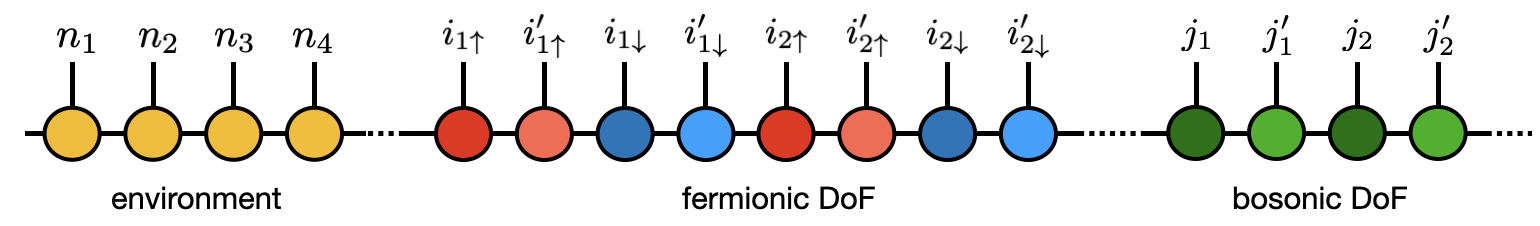
\includegraphics[width=0.8\textwidth]{figs/Schematic_ordering.png}
\end{figure}
\end{document}




